\documentclass[aps,prl,twocolumn,groupedaddress]{revtex4-1}
\usepackage{graphicx}

\begin{document}
\title{Optical Pumping and Magnetic Resonance}
\author{Dongwon Han}
\author{Kevin R. Wood}
%\email[]{kevin.wood@stonybrook.edu}
%\thanks{}
%\altaffiliation{}
\affiliation{Stony Brook University}

%Collaboration name if desired (requires use of superscriptaddress
%option in \documentclass). \noaffiliation is required (may also be
%used with the \author command).
%\collaboration can be followed by \email, \homepage, \thanks as well.
%\collaboration{}
%\noaffiliation

\date{\today}

\begin{abstract}
% insert abstract here
\end{abstract}

\maketitle

% body of paper here - Use proper section commands
% References should be done using the \cite, \ref, and \label commands
\section{Introduction}
Rubidium (Rb) is an alkali metal with atomic number $Z=37$.
Neutral states contain four entirely filled electron shells with no net angular moment and a single valence electron.
In its ground state, the valence electron carries no orbital angular momentum: $5^{2}S_{1/2}$.
It its first exited state, the valence electron carries one quanta of orbital angular momentum which can either align or anti-align with its spin contribution: $5^{2}P_{1/2}$ or $5^{2}P_{3/2}$. %"align or anti-align" probably isn't the best way to say this...

The energy splitting of the $5^{2}S$ and $5^{2}P$ states due to the Coulomb interaction with the nucleus on on the order of a few electron-volts.  The degeneracy of the first excited state is lifted by the spin-orbit coupling

\section{Review of Previous Work}
\section{Experimental Set-up}
\section{Measurements}

\begin{figure}
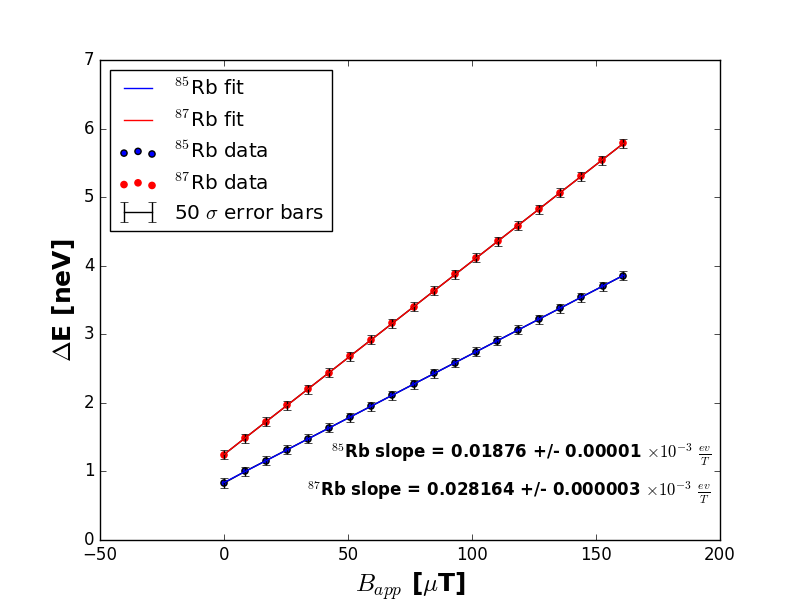
\includegraphics[width=\columnwidth]{magmom-verterr.png}
\caption{\label{MagMom} Measurement of the magnetic moment of $^{85}$Rb and $^{85}$Rb.}
\end{figure}

\section{Theoretical Model}
\section{Comparison of Data and Theoretical Model}
\section{Discussion and Conclusions}
\section{Author Contributions}
% Put \label in argument of \section for cross-referencing
%\section{\label{}}

\bibliography{basename of .bib file}

\end{document}